\begin{frame}{Aufbau - Architektur}

\begin{center}
\scalebox{0.75}{
\begin{tikzpicture}[scale=.6,database/.style={
      cylinder,
      cylinder uses custom fill,
      cylinder body fill=lblue,
      cylinder end fill=lblue,
      shape border rotate=90,
      aspect=0.25,
      align=center,
      draw
    }]
    

\definecolor{silver}{RGB}{158,158,169}
\definecolor{midgray}{rgb}{.35,.35,.35}
\definecolor{lightsilver}{RGB}{221,221,232}
\definecolor{lblue}{RGB}{210,220,250}
\definecolor{mblue}{RGB}{165,190,225}
\definecolor{dblue}{RGB}{0,70,117}
\definecolor{lgreen}{RGB}{200,245,185}
\definecolor{mgreen}{RGB}{190,225,165}
\definecolor{mred}{RGB}{225,190,165}
\definecolor{dgreen}{RGB}{40,135,40}
\definecolor{dred}{RGB}{135,40,40}

\visible<1>{
\draw[-,dashed,semithick,midgray] (8.5,-7.75) -- (-4,-7.75);
\draw[-,dashed,semithick,midgray] (8.5,3) -- (8.5,-7.75) -- (11.5,-10.75);
\node[draw=none,silver] at (6.75,-6.75) {\underline{TMetrics}};
\node[draw=none,silver] at (10.65,-6.75) {\underline{Data Origin}};
\node[draw=none,silver] at (6.75,-8.75) {\underline{User}};
}
\visible<2->{
\draw[-,dashed,semithick,silver] (8.5,-7.75) -- (-4,-7.75);
\draw[-,dashed,semithick,silver] (8.5,3) -- (8.5,-7.75) -- (11.5,-10.75);
\node[draw=none,lightsilver] at (6.75,-6.75) {\underline{TMetrics}};
\node[draw=none,lightsilver] at (10.65,-6.75) {\underline{Data Origin}};
\node[draw=none,lightsilver] at (6.75,-8.75) {\underline{User}};
}

\node[fill=mred,draw=black,font=\small, minimum height=1cm, minimum width= 2.5cm] (fe) at (0, -10.5) {{\only<3->{JS} Frontend}};
\node[ellipse,fill=mblue,draw=black,font=\small, minimum height=1cm, minimum width= 2.5cm] (tw) at (13, 0) {Twitter};

\visible<1>{
\node[fill=lblue,draw=black,minimum width=2.5cm, minimum height=1.5cm, font=\small] (tm) at (0,0) {TMetrics};
\draw[->,semithick,>=stealth',shorten >=1pt] (tw) -- (tm);
\draw[->,semithick,>=stealth',shorten >=1pt] (tm) -- (fe);
}


\visible<2->{
\node[database, minimum width=2cm, minimum height=1.5cm, font=\small] (db) at (0,0) { { \visible<3->{MySQL} } \\ DB}; %
\node[fill=lblue,draw=black,font=\small, minimum height=1cm, minimum width= 2.5cm,align=center] (rs) at (0, -3) {{\only<2>{Webservice}} \only<3->{Restservice \\ Tomcat}}; %
\node[fill=lblue,draw=black,font=\small, minimum height=1cm, minimum width= 2.5cm] (de) at (5.5, 0) {Daemon};
}

\visible<2>{
\draw[->,semithick,>=stealth',shorten >=1pt] (tw) -- (de);
\draw[->,semithick,>=stealth',shorten >=1pt] (de) -- (db);
\draw[->,semithick,>=stealth',shorten >=1pt] (db) -- (rs);
\draw[->,semithick,>=stealth',shorten >=1pt] (rs) -- (fe);
}

\visible<3->{
\draw[->,semithick,>=stealth',shorten >=1pt] (tw) -- (de) node[midway,above,font=\scriptsize] {Twitter4J};
\draw[<->,semithick,>=stealth',shorten >=1pt,shorten <=1pt] (de) -- (db) node[midway,above,font=\scriptsize] {JDBC};
\draw[<->,semithick,>=stealth',shorten >=1pt,shorten <=1pt] (db) -- (rs) node[midway,left,font=\scriptsize] {JDBC};
}

\visible<3>{
\draw[<->,semithick,>=stealth',shorten <=1pt,shorten >=1pt] (rs) -- (fe);
}

\visible<4->{
\node[fill=lblue,draw=black,font=\small, minimum height=1cm, minimum width= 2.5cm,align=center] (ap) at (0, -6) {HTTP Apache};
}

\visible<4>{
\draw[<->,semithick,>=stealth',shorten <=1pt,shorten >=1pt] (rs) -- (ap);
\draw[<->,semithick,>=stealth',shorten <=1pt,shorten >=1pt] (ap) -- (fe);
}

\visible<5->{
\draw[->,semithick,>=stealth',shorten >=1pt] ([xshift=-0.5cm]ap.south) -- ([xshift=-0.5cm,yshift=1.5cm]fe.north) node[midway,left,align=right,font=\scriptsize] {Frontend Code};
\draw[<-,semithick,>=stealth',shorten <=1pt] ([xshift=0.5cm]ap.south) -- ([xshift=0.5cm]fe.north) node[midway,right,align=left,font=\scriptsize] {HTTP Requests};
\draw[->,semithick,>=stealth',shorten >=1pt] ([xshift=-0.25cm]rs.south) -- ([xshift=-0.25cm]ap.north) node[midway,left,font=\scriptsize] {Replies (JSON)};
\draw[<-,semithick,>=stealth',shorten <=1pt] ([xshift=0.25cm]rs.south) -- ([xshift=0.25cm]ap.north) node[midway,right,align=left,font=\scriptsize] {HTTP Requests};
\draw[->,semithick,>=stealth',shorten >=1pt] ([xshift=0cm]ap.south) -- ([xshift=0cm]fe.north) node[midway,left,align=right,font=\scriptsize] {\ \\ \ \\ Replies (JSON)};
}

\visible<6->{
\draw[<-,semithick,>=stealth',shorten <=1pt] (rs) -- (de) node[midway,right,font=\scriptsize] {SentimentModel};
}

\visible<7->{
\node[ellipse,fill=mgreen,draw=black,align=center,font=\small, minimum height=1cm, minimum width= 2.5cm] (ne) at (13, -3) {Google News \\ Bing Web \\ Bing News};
\draw[<-,semithick,>=stealth',shorten <=1pt] (rs) -- (ne) node[midway,above,font=\scriptsize] {RSS Feeds};
}


\end{tikzpicture}
}
\end{center}

\end{frame}

\begin{frame}{Aufbau - Frontend}
    \begin{itemize}
        \item Darstellung im Browser 
        \item Verwendung verschiedener Frameworks (jQuery, Bootstrap, Highcharts)
        \item Darstellung mittels HTML5 und CSS3
    \end{itemize}
\end{frame}

\begin{frame}
    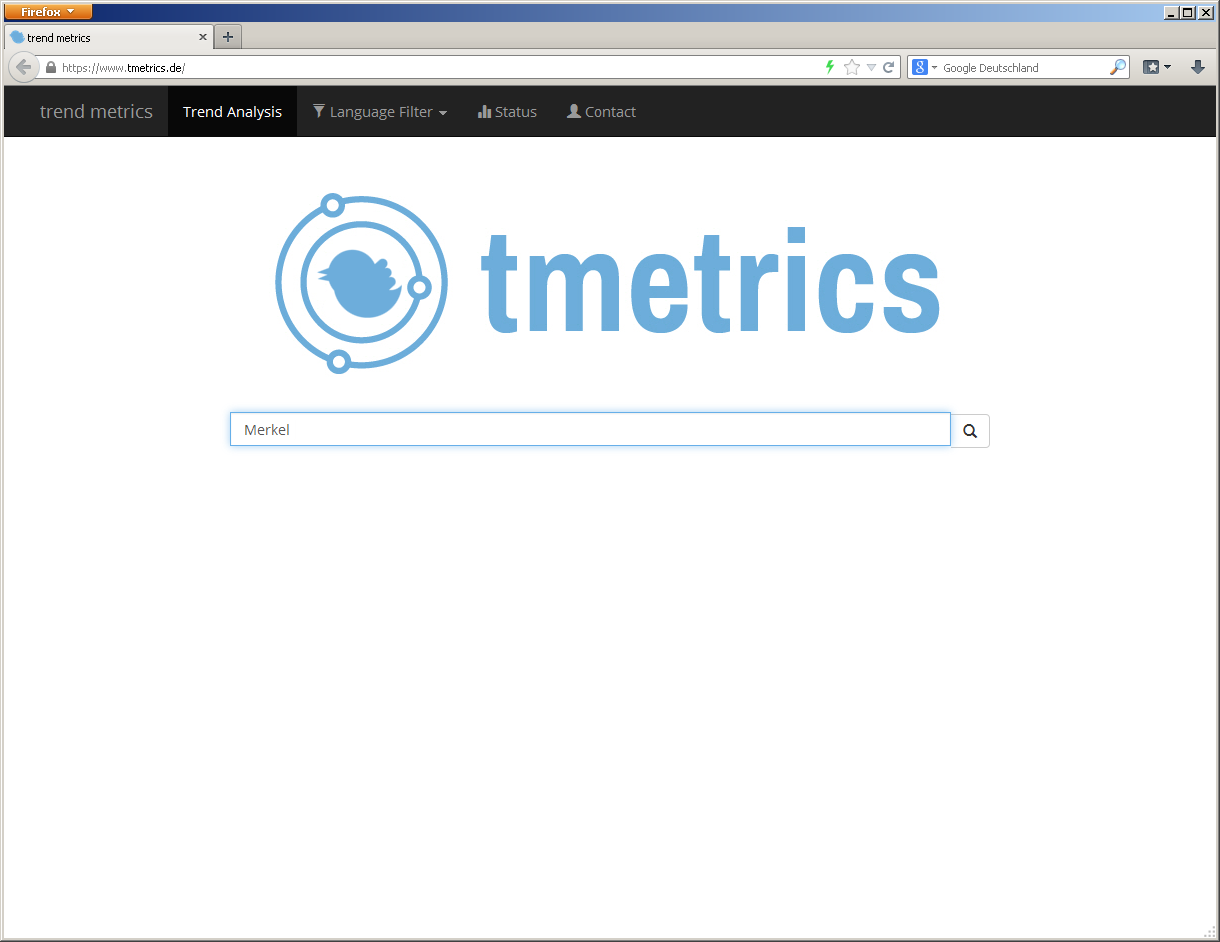
\includegraphics[width=0.926\textwidth]{../img/shots/01.png}
\end{frame}

\begin{frame}
    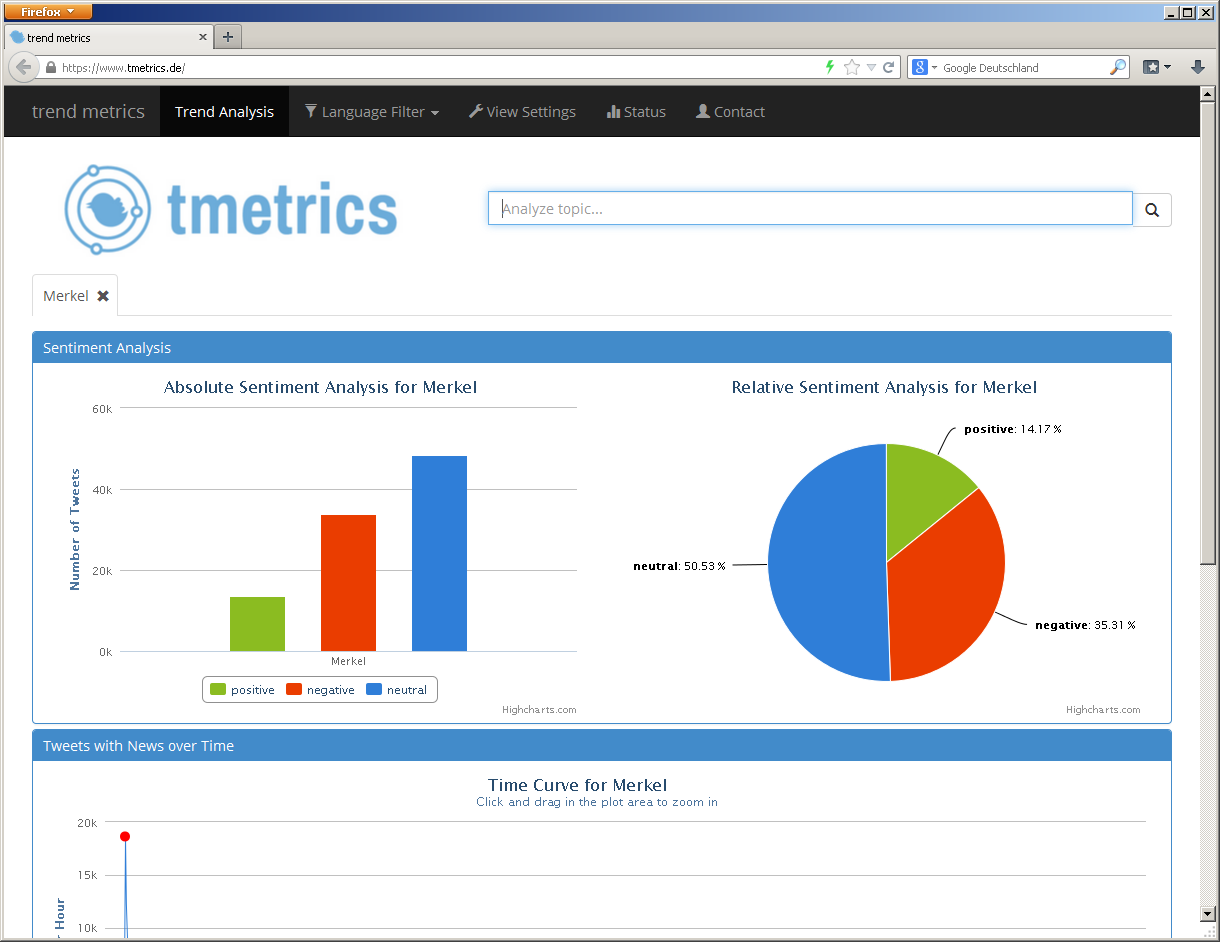
\includegraphics[width=0.926\textwidth]{../img/shots/02.png}
\end{frame}

\begin{frame}
    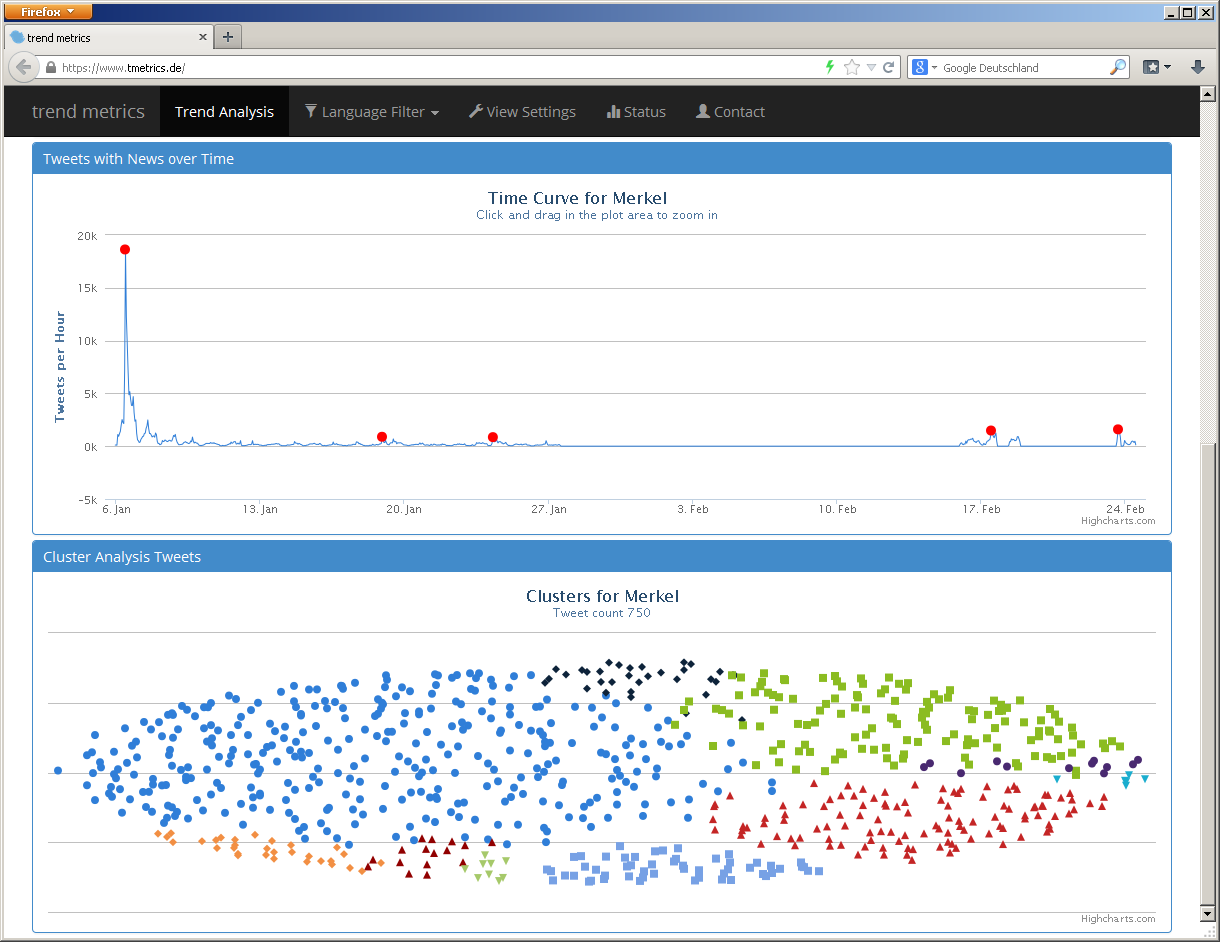
\includegraphics[width=0.926\textwidth]{../img/shots/03.png}
\end{frame}

\begin{frame}
    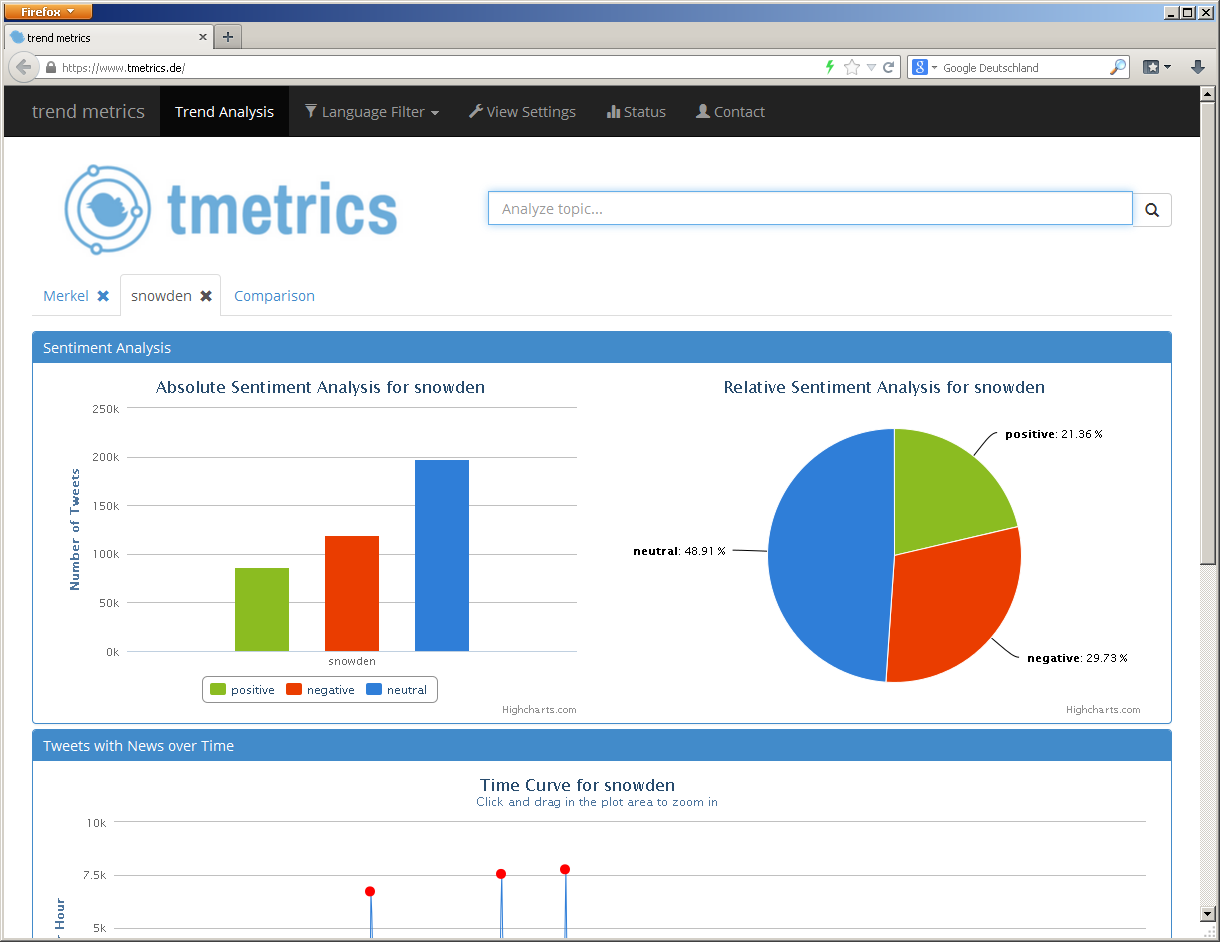
\includegraphics[width=0.926\textwidth]{../img/shots/04.png}
\end{frame}

\begin{frame}
    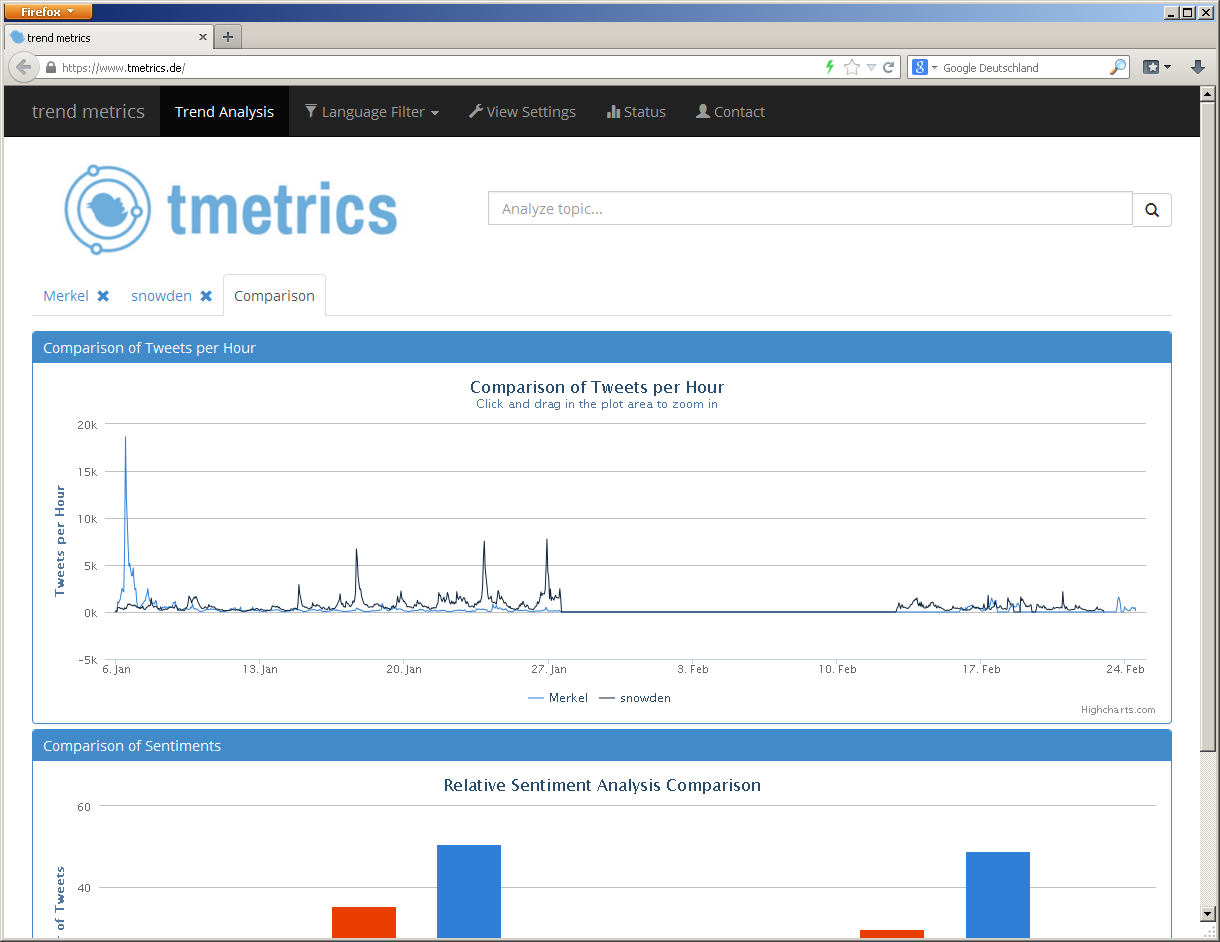
\includegraphics[width=0.926\textwidth]{../img/shots/06.png}
\end{frame}

\begin{frame}
    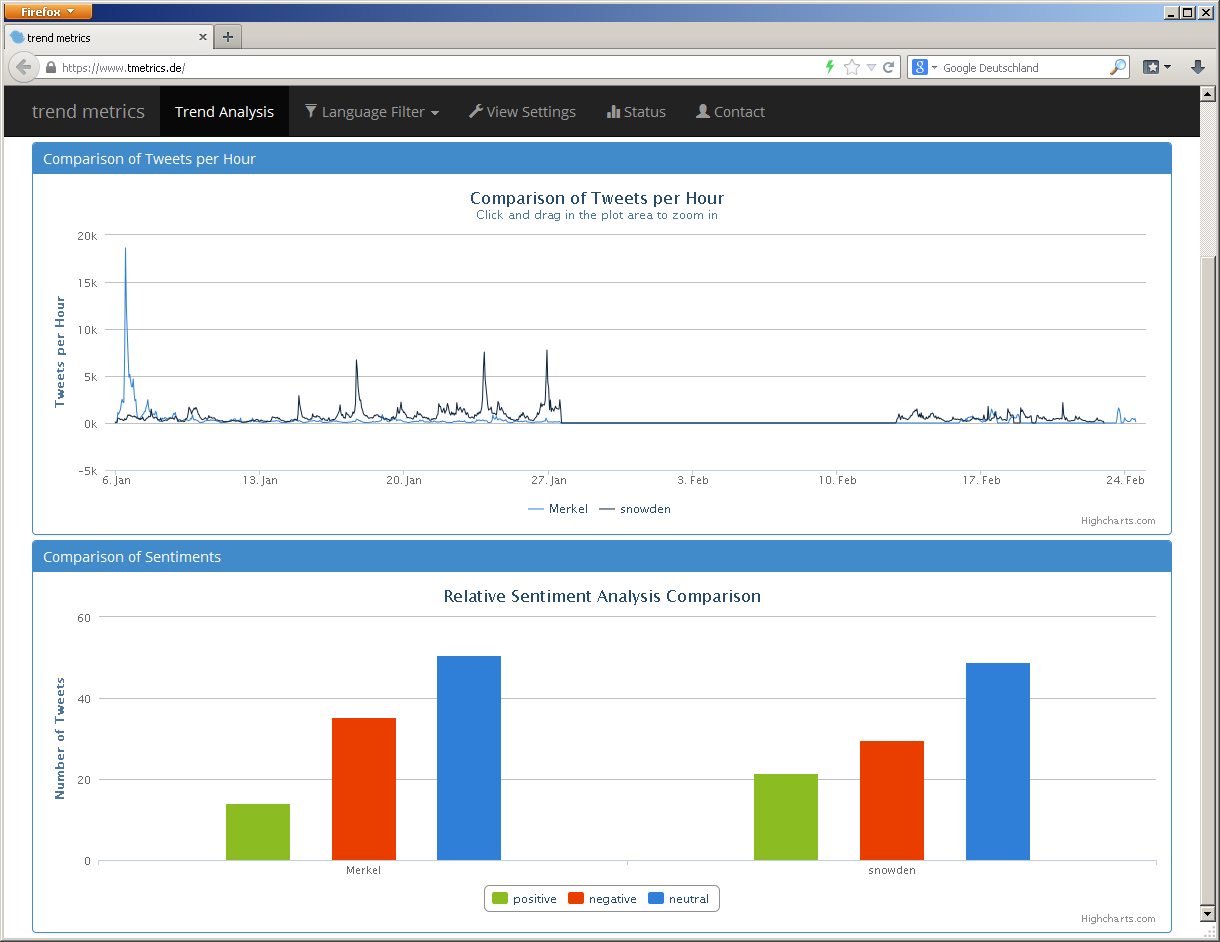
\includegraphics[width=0.926\textwidth]{../img/shots/07.png}
\end{frame}

\begin{frame}{Aufbau - Frontend}
    \begin{itemize}
        \item Einfach und intuitiv zu bedienen
        \item Reiter und Zoom sind bekannte Bedienkonzepte
        \item Anzeigebereich nicht überladen, sondern übersichtlich gehalten
        \item Weitere Details zur Funktionalität folgen in der Demonstration
    \end{itemize}
\end{frame}
